\section{\smyrna\ Controls}
\label{sec:controls}

In this section, we describe the various controls making up 
the \smyrna\ interface. Figure~\ref{fig:main} shows an example of
the main \smyrna\ display.

\begin{figure}[ht] 
\begin{center}
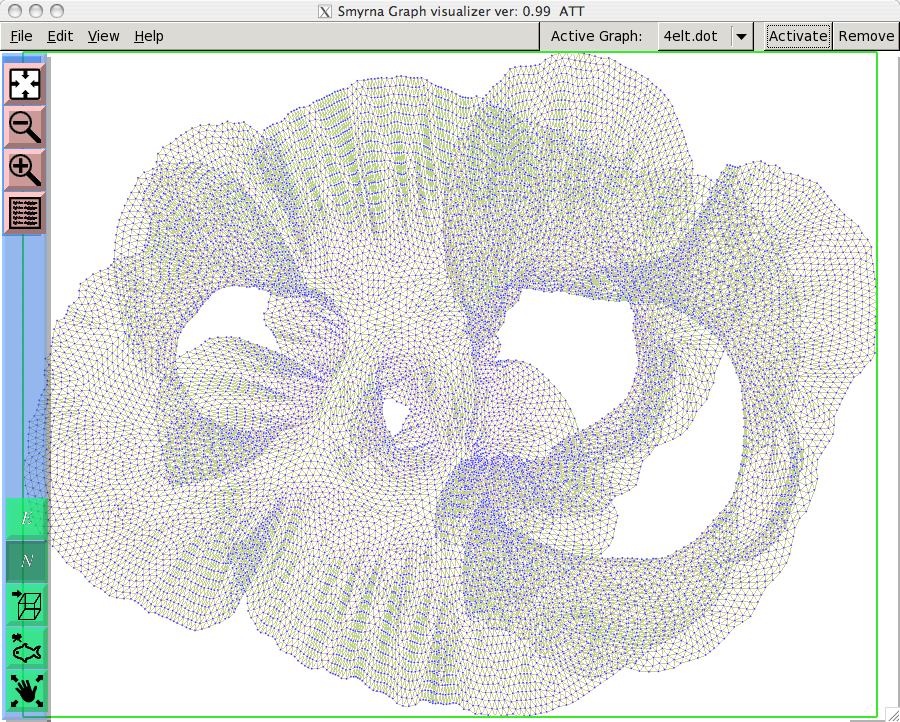
\includegraphics[scale=.3]{figures/smyrna.png}
\caption{\small Typical \smyrna\ view.}
\label{fig:main} 
\end{center}
\end{figure}


Across the top of the main window, there is a fairly standard menu bar. 
The {\tt File} pull-down menus offers the choices {\bf Open}, {\bf Save},
{\bf Save As} and {\bf Quit}. These should be self-explanatory.
The {\tt View} menu allows you to make the console window a subwindow of the
main \smyrna\ window. 
\begin{comment}
 As open and hide are mutually exclusive, this menu should
be made dynamic, or the control should be done as a toggle.
\end{comment}
The {\tt View} menu also lets you open the Node List widget, which 
gives information about the currently selected nodes.
This is considered in detail in Section~\ref{sec:nodelist}.
The {\tt Help} menu provides access to information about using \smyrna\ {\bf but at
present does nothing}.
%The {\tt Select} menu provides shortcuts for selecting and unselecting large parts
%of the the graph, such as all nodes.

The {\tt Edit} menu consists of two items: {\bf Smyrna Settings} and {\bf Attributes}.
The first activates the \smyrna\ Settings Widget described in
Section~\ref{sec:settings}. This widget provides access to the parameters controlling
\smyrna's behavior, as well as providing some high-level manipulation of the graph.
The second provides a short-hand access to the Attributes tab (Section~\ref{sec:attr})
of the Settings Widget. 

On the right of the menu bar are controls for handling the loaded graphs.
The currently active graph is shown. The names of all available graphs are provided in the
associated pull-down menu. To switch between graphs, the user can pick another graph from
the menu, then click on the {\tt Activate} button. Alternatively, clicking on the {\tt Remove}
button closes the graph. {\bf This doesn't appear to work.}

The top buttons along the left of the main window serve as simple controls for
certain common actions. 
\begin{description}
\item[
\includegraphics{figures/center.png}]
The top button is used to re-center the display. 
\item[
\includegraphics{figures/zoomin.png} 
\includegraphics{figures/zoomout.png}]
The next two buttons allow you to zoom in and
out. 
\item[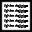
\includegraphics{figures/details.png}]
The fourth top button is yet another shortcut for opening the 
Attributes tab (Section~\ref{sec:attr}) in the Setting widget.
\end{description}

The bottom buttons are used to toggle between states in \smyrna.
\begin{description}
\item[E  N]
The top two, E and N, determine whether edges and nodes are selected when doing
an area selection. Programmatic selection or single selection by mouse still works even
if these are unset.
\item[
\includegraphics{figures/2D.png} 
\includegraphics{figures/3D.png}]
The buttons toggle between 2D and 3D display modes. 
If the {\tt pos} attributes of the nodes has only two coordinates, the
z value is taken to be 0, and the graph appears in the XY plane.
\item[
\includegraphics{figures/fisheye.png} 
\includegraphics{figures/no_fisheye.png}]
The fish buttons toggle between the normal and topological fisheye views (Section~\ref{sec:topfish}).
\item[
\includegraphics{figures/pan.png}]
The last button unselects all selected objects. 
\begin{comment}
This makes me feel this button should be at the top.
\end{comment}
\end{description}

\subsection{\smyrna\ Settings Widget}
\label{sec:settings}
This is the main control panel for controlling the display parameters in
\smyrna. It also provides two tabs for interacting with the graph: a high-level
interface for dealing with graph attributes, and a general-purpose interface
for applying \gvpr\ on the graph. We discuss each tab individually in
the following subsections.

Note that is necessary to click on the {\tt Apply} button to cause the changes to
take effect. 
\begin{comment}
Why not make each change immediate?
\end{comment}

\subsubsection{General Settings}
\label{sec:general}
The General Settings tab is shown in Figure~\ref{fig:general}.
It provides control control over the default color schemes, and whether
or not nodes and edges are drawn or can be selected.
Clicking on one of the colors brings up a color selection widget that allows
you to modify the color.
\begin{figure}[ht]
\begin{center}
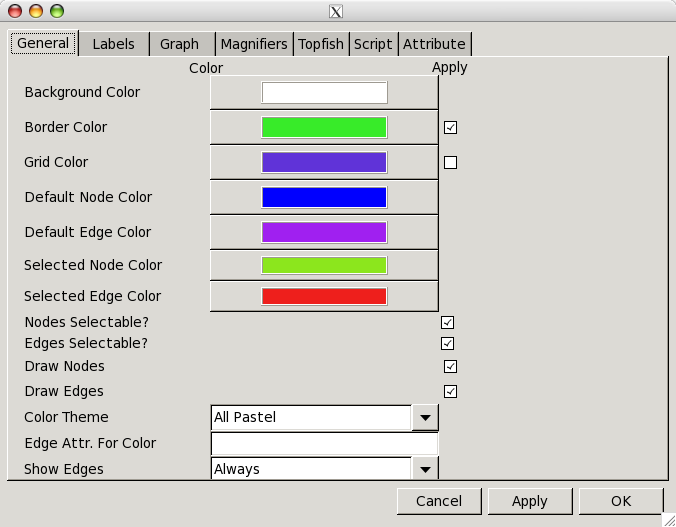
\includegraphics[scale=.5]{figures/general.png}
\caption{\small The General Settings tab.}
\label{fig:general}
\end{center}
\end{figure}
\begin{description}
\item[Background Color] 
Specifies the background color of the window.
\item[Border Color] 
Specifies the border color.
If enabled, \smyrna\ draws a rectangle about the graph to indicate its limits.
This attribute specifies what color is used.
\item[Grid Color] specifies the color of grid points.
If enabled, \smyrna\ draws an array of grid points behind the graph.
\item[Default Node Color] gives the color used to draw nodes, unless specified explicitly
in the input graph.
\item[Default Edge Color] gives the color used to draw edges, unless specified explicitly
in the input graph or a color theme is selected.
\item[Selected Node Color] specifies the color used for selected nodes.
\item[Selected Edge Color] specifies the color used for selected edges.
\end{description}

This tab also provides check boxes to enable or disable various properties.
These can be used to turn off the drawing of nodes, edges, the border or the grid.
In addition, the ability to select nodes or edges using the GUI can be disabled.

\smyrna\ provides a collection of color themes which can be selected using the {\tt Color Theme}
menu. This specifies a color theme used to color edges with no color attribute. Edge color
calculations are based on an edge's {\em len} attribute. A different edge attribute can
be specified using the {\tt Edge Attr. for Color} text box. 
\begin{comment}
This doesn't appear to be
implemented yet? Also, how does one turn of the color themes, so that the default edge color
is used?
\end{comment}

The {\tt Show Edges} menu can be used to determine when edges are drawn. Normally, an edge
is drawn if any part of it appears within the view windows. Sometimes, for clarity or efficiency,
it is better to only draw those edges with at least one node with the view.

\subsubsection{Labels}
\label{subsubsec:labels}
The Labels tab is shown in Figure~\ref{fig:labels}.
This tab provides control over labels used in \smyrna.
\begin{figure}[ht]
\begin{center}
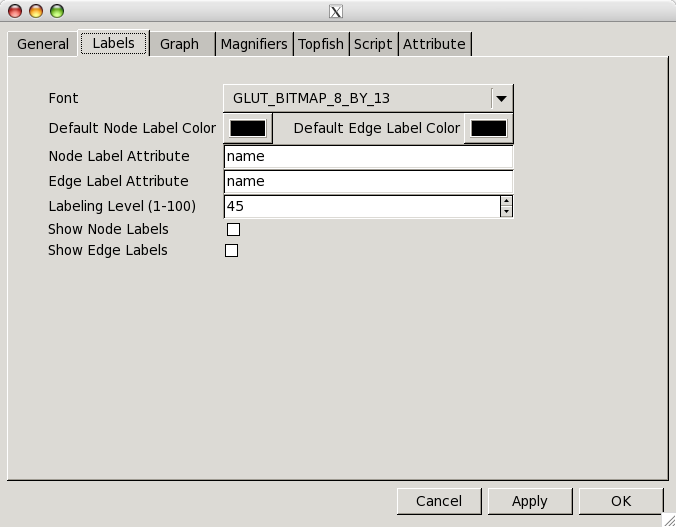
\includegraphics[scale=.5]{figures/labels.png}
\caption{\small The Labels tab.}
\label{fig:labels}
\end{center}
\end{figure}
The {\tt Font} menu can be used to set the face and standard size of the OpenGL font used to
display text labels.
The {\tt Default Node Label Color} and {\tt Default Edge Label Color} items can be used to
specify which colors are used for node and edge labels, respectively.

The user can tailor what attribute is used as the label for nodes and edges. This is done via
the {\tt Node Label Attribute} and {\tt Edge Label Attribute} text boxes. For example,
a graph representing Internet communication may benefit from using a node attribute such
as {\it IPaddress} or {\it hostname}. Note that,
by default, the label comes from the pseudo-attribute {\it name}. For nodes, this is the
name of the node; for edges, the name is constructed from the names of its head and tail nodes.
\begin{comment}
I wonder if label may be a better and more
appropriate default attribute to use, since if the graph has been processed, the label will be
node name. Also, when are labels shown? 
\end{comment}

Labels are shown when an object is selected. In addition, if the Show Node Labels box is checked,
labels are displayed for all nodes whenever one zooms in close enough. Close enough is determined
by the Labeling Level widget. The smaller the number, the sooner labels appear as you zoom in.
 
\subsubsection{Graph}
The Graph tab is shown in Figure~\ref{fig:graph}.
With this tab, the user can affect more technical aspects of the graph view.
\begin{figure}[ht]
\begin{center}
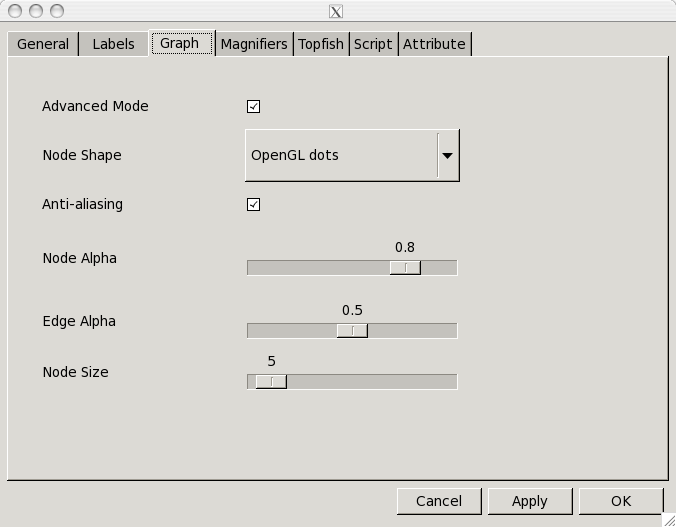
\includegraphics[scale=.5]{figures/graph.png}
\caption{\small The Graph tab.}
\label{fig:graph}
\end{center}
\end{figure}
The {\tt Node Shape} menu allows the user to specify how nodes are drawn.
\begin{description}
\item[OpenGL dots] Nodes are drawn as filled circles as efficiently as possible. All nodes
will have the same size.
\item[Spherical] Nodes are drawn using OpenGL spheres. The advantage over OpenGL dots is that
each node can have its own size specified by the size attribute. The disadvantage is that it is not
as efficient.
\item[Custom] At present, the choice is not implemented.
\end{description}

This tab provides three sliders. The {\tt Node Alpha} and {\tt Edge Alpha} 
sliders control the transparency of nodes and edges. Set to 1.0, the object is opaque;
set to 0, the object is invisible. A typical use would be to set the edge alpha to a small
value rather than to turn off edge drawing entirely. The edges would still be visible, but
would obscure the drawing as much. 
These values are multiplied with any alpha valued supplied with an edge's or node's color.
The {\tt Node Size} slider can be used to uniformly
scale the node size. Note that the node sliders have no effect for custom nodes.

The {\tt Advanced Mode} and {\tt Anti-aliasing} check boxes toggle the advanced user mode 
\begin{comment}
 What does this mean?
\end{comment}
and the use of anti-aliasing.


\subsubsection{Magnifier Settings}
The Magnifiers tab is shown in Figure~\ref{fig:magnifier}.
This controls the magnifying glass parameters.
\begin{figure}[ht]
\begin{center}

\includegraphics[scale=.5]{figures/magnifier.png}
\caption{\small The Magnifiers tab.}
\label{fig:magnifier}
\end{center}
\end{figure}
The radius of the fisheye magnifier is specified using the {\tt Radius} field.
The {\tt Distortion} field allows you control the distortion in the lens. Larger distortion
causes greater magnification.
\begin{comment}
What do the width, height and Zoom X fields do, and why are their boxes so different in size?
\end{comment}


\subsubsection{Topfish Settings}
The Topfish tab is shown in Figure~\ref{fig:topfish}.
This allows you to specify the parameters associated with a topological fisheye view of the
graph as discussed in Section~\ref{sec:topfish}.
\begin{figure}[ht]
\begin{center}
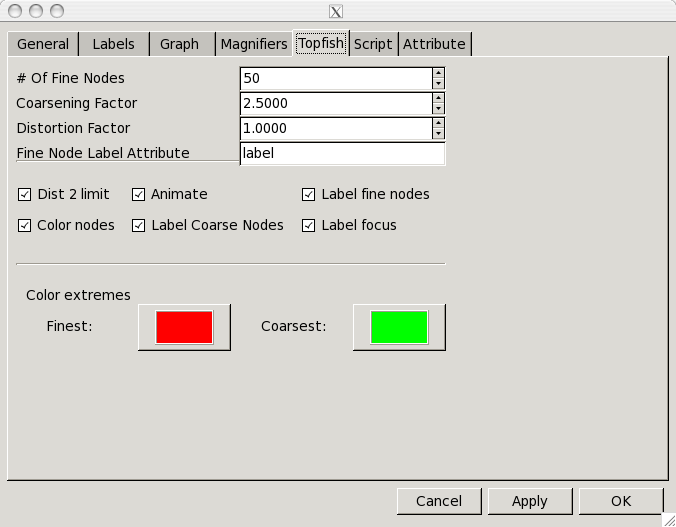
\includegraphics[scale=.5]{figures/topfish.png}
\caption{\small The Topfish tab.}
\label{fig:topfish}
\end{center}
\end{figure}
The {\tt \# Of Fine Nodes} field allows the user to set the number of the fine nodes 
The {Fine Node Label Attribute} indicates what node attribute is used to label fine nodes.
The {\tt Coarsening factor} and {\tt Distortion Factor} fields control some technical
parameters of the view; refer to the paper for more details.

There are six check boxes.
\begin{description}
\item[Dist 2 Limit] Distance to limit value of the algorithm  {\bf What does this mean?}
\item[Animate] Toggles whether animation is used to handle the transition from an old focus to
a new focus. Although more expensive, animation helps to preserve the mental map of the graph.
\item[Label Fine Nodes] Indicates whether fine nodes are labeled.
\item[Color nodes]  {\bf What does this do?}
\item[Label Coarse Nodes] {\bf What does this do?}
\item[Label Focus] Indicates whether the focus node is labeled. The focus node label is
displayed prominently whether or not the labeling of fine nodes is enabled.
\end{description}

The two {\tt Color extremes} widgets allow you to set the colors used for the finest
and coarsest nodes. Colors of intermediate nodes are interpolated between these two colors.

\subsubsection{Applying \gvpr}
\label{sec:gvprtab}
The Script tab is shown in Figure~\ref{fig:gvpr}.
This is the main control for using \gvpr\ scripts to manipulate the active graph
as discussed in Section~\ref{sec:gvpr}.
\begin{figure}[ht]
\begin{center}
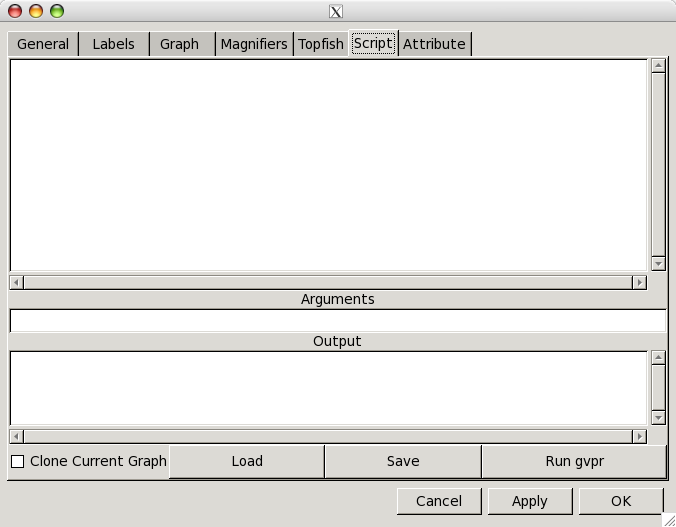
\includegraphics[scale=.5]{figures/gvpr.png}
\caption{\small The \gvpr\ tab.}
\label{fig:gvpr}
\end{center}
\end{figure}
The top text window can be used to enter and edit a \gvpr\ script. By then clicking on 
the {\tt Run gvpr} button, the script is run on the active graph. As usual, to update
smyrna's data structures, you will need to click the {\tt Apply} (or {\tt OK}) button,
and then click on the main \smyrna\ window to cause the the display to be refreshed. 
\begin{comment}
Can this be avoided?
\end{comment}

By default, any changes are done directly to the active graph. Often, this is appropriate.
During exploratory data analysis, though, the user may wish to keep the original graph unaltered
in order to return to it later. Rather than trying to undo any changes made, it is simpler to
mark the {\tt Clone Current Graph} checkbox. In this case, a clone of the original graph is made.
Then, the \gvpr\ is applied to the cloned graph, which then becomes the new active graph. The
original graph can be retrieved using the {\tt Active Graph} menu at the top of the main
\smyrna\ window. The obvious drawbacks to this mode are that there is the extra time needed to
clone the graph, and the extra memory use for each copy.

A \gvpr\ script accepts arguments, which are available via the {\tt ARGV[]} array. Normally, these
would be provided on the command line. Here, the user can use the middle {\tt Arguments} text
window to supply these.

In addition to manipulating a graph, a \gvpr\ script can also perform I/O to a {\tt stdout} stream. 
This output appears
in the console window, which is labeled {\tt Output}. The console window opened as part of the
main \smyrna\ window using the {\tt View} menu is another view of the same stream.  

Finally, the {\tt Load} and {\tt Save} buttons support the re-use of \gvpr\ scripts.
Specifically, the {\tt Load} button can be used to read in a file, whose contents are stored 
in the \gvpr\ script text window, overwriting any previously stored script. Conversely, the
{\tt Save} button can be used to write the contents of the script text window into a file
for later use.

\subsubsection{Setting Attributes}
\label{sec:attr}
Manipulating attributes is a common task when using \smyrna. Any such operations can be done
using \gvpr. However, it seems reasonable to support this activity with a simpler interface.
The purpose of the Attribute tab is to provide this interface, though it should be noted that
the actual work is done using \gvpr.

Figure~\ref{fig:attr1} shows the initial state when the Attributes tab is opened.
Note that the caption indicates that some collection of nodes and edges has been selected.
	\begin{figure}[ht]
	\begin{center}
	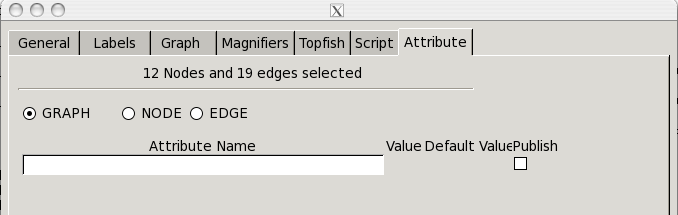
\includegraphics[scale=.5]{figures/attr1.png}
\caption{\small The Attribute tab.}
\label{fig:attr1}
\end{center}
\end{figure}
To start, use the radio buttons to specify what type of 
graph object you wish to work with. Then type in the attribute's name in the
{\tt Attribute Name} field. As you type, the tab interface changes dynamically in
response to your typing,
giving feedback concerning what it knows about available attributes. If what you have
typed is the prefix of a known attribute, all attributes with that prefix will appear
in a list below. In Figure~\ref{fig:attr2}, the character 's' causes the various
known node attributes starting with 's' to be shown.
\begin{figure}[ht]
\begin{center}
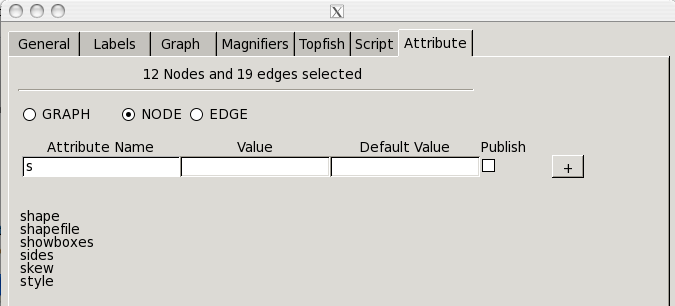
\includegraphics[scale=.5]{figures/attr2.png}
\caption{\small Typing in the Attribute tab.}
\label{fig:attr2}
\end{center}
\end{figure}

\begin{description}
\item[Searching and modifying attributes]
If the current text fully matches a known attribute,
the background color of the {\tt Attribute Name} field will appear in green. 
In the example shown in Figure~\ref{fig:attr3}, the shape attribute has been
recognized and the default value is shown. 
In addition, you will see three additional buttons: {\tt Apply}, {\tt Apply All} and {\tt Search}.

\begin{figure}[ht]
\begin{center}
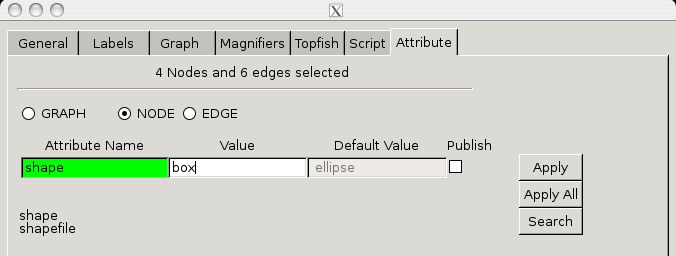
\includegraphics[scale=.5]{figures/attr3.png}
\caption{\small A recognized attribute.}
\label{fig:attr3}
\end{center}
\end{figure}

The {\tt Apply} button is used to replace the attribute values of selected objects of the 
specified object type. In our example, we have chosen the {\tt shape} attribute, 
and have specified a value of {\tt box} in the Value field. If we then click the {\tt Apply},
\smyrna\ will set the shape value of all selected nodes to the given value.
Note that if no objects have been selected, the {\tt Apply} button will not be active.

The {\tt Apply All} button is identical to the {\tt Apply} button except that the
attribute change is performed on all objects, not just the selected ones.

The {\tt Search} button is used to select objects of the specified object type based on
attribute values specified by regular expressions.
For example, suppose that you have a network graph with IP addresses 
attached to each node. You can type {\tt IP} in the attribute name box, {\tt 10.*} in the
value box, and click on the {\tt Search} button. 
This will select all nodes whose IP address begins with {\tt 10.}. Regular expression
matching is, obviously, based on the regular expressions supported in \gvpr.

\item[Adding new attributes]
If, as you type, the attribute name is not currently set in the graph for the specified object type,
the Attribute Name field will be red and
a button with a plus sign ('+') will appear, as in Figure~\ref{fig:attr4}.
You can then type in a value into the {\tt Default Value} field, click on the '+' button and
the appropriate attribute will be created with the given default value, and all objects
of the given type that value for the attribute.
Here, we have specified a default
value of "yes" in the Default Value field. If we now click on the '+' button on the right,
\smyrna\ will create this new node attribute.

\end{description}

\begin{figure}[ht]
\begin{center}
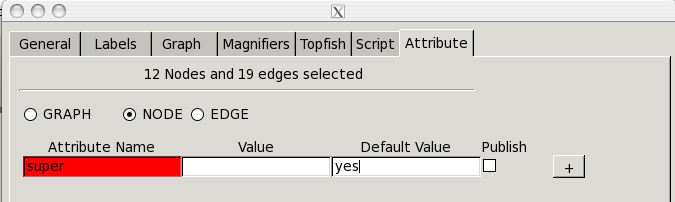
\includegraphics[scale=.5]{figures/attr4.png}
\caption{\small An unknown attribute.}
\label{fig:attr4}
\end{center}
\end{figure}

\subsection{The Node List Widget}
\label{sec:nodelist}
It is often useful to be able to focus on certain nodes, and look at some of their associated attributes. 
This can be done using \gvpr (\ref{sec:gvprtab}), but this type of query is important enough that \smyrna\
provides the special-purpose Node List widget. This is opened by using the {\tt Edit} menu.
Figure~\ref{fig:nodelist} shows a typical view of the widget. It lists all of the currently selected nodes.
Selection could have been down by clicking on the nodes, sweeping out a region, or via \gvpr.
\begin{figure}[ht]
\begin{center}
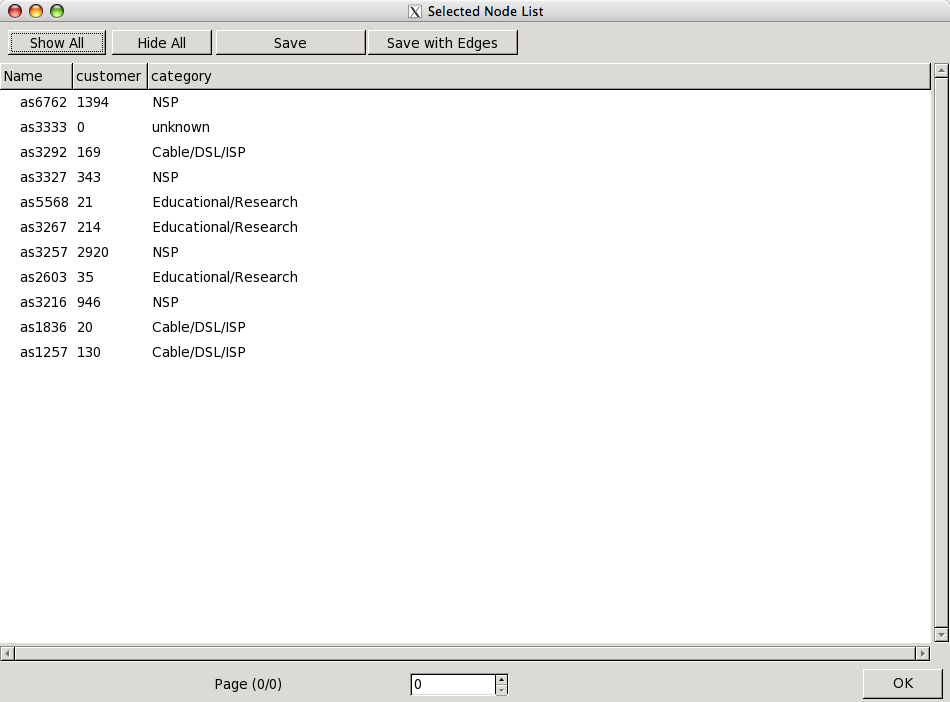
\includegraphics[scale=.35]{figures/nodelist.png}
\caption{\small The Node List widget.}
\label{fig:nodelist}
\end{center}
\end{figure}
The list always gives the names of the selected nodes. You can specify additional attributes to be
displayed by setting the graph's {\tt datacolumns} attribute, which is a comma-separated list of the
desired attribute names. Thus, in the example shown, the graph has {\tt datacolumns="category,customer"}.
To select new columns, just run \gvpr. For example, to switch the current two columns and add the
{\tt tier} attribute, you would run the \gvpr\ script
\begin{verbatim}
BEG_G{datacolumns="customer,category,tier"}
\end{verbatim}
Note that, at present, you will need to close and then re-open the Node List widget to get the new columns.

The widget provides four buttons that can sometimes be useful in this context. The subgraph may be
interesting enough that you wish to view it off-line. By clicking the {\tt Save} button, you can save
the nodes as a separate graph. The {\tt Save with Edges} button, the graph saved with the selected nodes
and all edges in the original graph between two selected nodes. The {\tt Hide All} button will make all of 
the selected nodes invisible; the {\tt Show All} button makes them all visible.
